%!TEX root = ../../../super_main.tex
\subsection{Request Handling}
\label{sub:request_handling}
The entry point for the Laravel framework is through the \mono{index.php}, which is a file that comes with the framework out of the box. The framework after receiving a request create its own \mono{Request} object. This request object is then sent to a handler, which initiates the flow shown in \figref{fig:laravel_flow}.

\begin{figure}[!htbp]
    \centering
    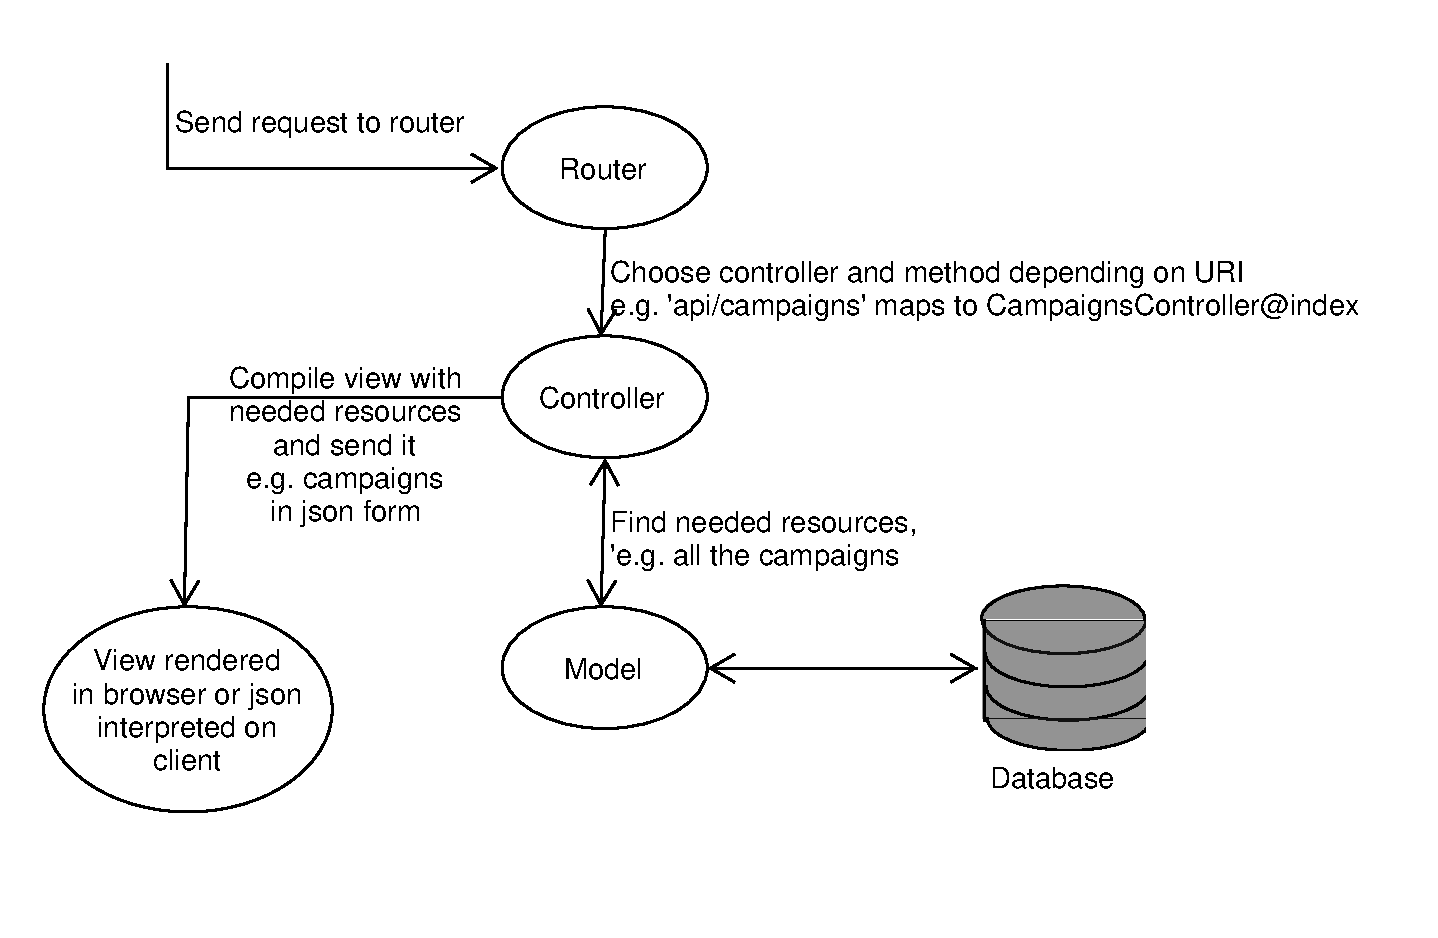
\includegraphics[width=0.7\textwidth]{graphic/architecture/laravel_flow.pdf}
    \caption{An illustration of how a request is traverses through Laravel.}
    \label{fig:laravel_flow}
\end{figure}
\FloatBarrier

Firstly the request is send to the router, which looks at the request URI and determines, depending on the URI, which controller-method should be called, retrieves any parameters captured by wildcards in the URI, and invoke the controller-method with these. It is then the controllers job to fetch the needed models from the database to create the requested view, which in the case of an API route will be a JSON response of the given models. The JSON response will then be interpreted by the Android client and the requested information will be shown to the user. 

\subsubsection{Directing Traffic}
\label{ssub:directing_traffic}
To enable the Laravel framework in the first place we need to direct the traffic to our server from a requested URL to the entry point for the Laravel framework, and there also is the problem that we as mentioned in \secref{sec:server} need to map four different server names to two different sites, namely the production site and the development site. To solve these problems we utilize NGINX. NGINX allows us to specify what is called virtual servers, which allows a single server to listen on different ports, but also allows us to serve different sites depending on the requested server name. Each virtual server has a list of server names associated to them, which is used to determine if the virtual server should handle the request or not, e.g. if a request is made to the URL, \mono{prod.local.element67.dk/api/campaigns}, the virtual server with the server name \mono{prod.local.element67.dk} in its list should handle it. 
Besides the server names, we can specify how the virtual server should process different requests. We can amongst other things specify where to look for the documents to serve by setting the document root or specify that the traffic always should be directed to the entry point for the Laravel framework, namely \mono{index.php}. 
\\\\
An example of how a request to \mono{prod.local.element67.dk/api/campaigns} is handled by our NGINX setup can be seen in \figref{fig:NGINX_workflow}. NGINX will when receiving such a request try to decide, which virtual server should handle the request. In our configuration we have a virtual server defined, which has the server names \mono{prod.local.element67.dk} and \mono{prod.global.element67.dk} attached to it. Therefore NGINX will choose this virtual server. Note that the document root is set to \mono{/var/www/datacollection-prod/public} in the configuration of this virtual server as in \figref{fig:NGINX_workflow}.
\\\\ %Should we mention the document root
Now the server knows what server it should utilize, however it should also determine how the requested URL should be served. For this purpose we can define what is called location directives inside the configuration file of the virtual server. A location directive consists of a rule to match the requested URI, as well as a body containing a strategy or further configuration of how to handle the request. NGINX will then decide which location directive's strategy should be used by finding the best matching location rule. In our configuration for the production server we have defined two different location directives, shown as \emph{location 1} and \emph{location 2} in \figref{fig:NGINX_workflow}. \emph{Location 1}'s rule describes the most general matcher possible, namely \mono{'/'}, and it will therefore act as a fall-back for all requests, whereas the second location is more specific with the rule, \mono{'\textasciitilde ~ \textbackslash .php'}, which is a regular expression rule (defined by the tilde prefix), that will match all requests made to PHP files. 
\\
\begin{figure}[!htbp]
    \centering
    \includegraphics[width=0.7\textwidth]{graphic/architecture/NGINX_workflow.pdf}
    \caption{An example of how a request could be handled by NGINX with our configuration.}
    \label{fig:NGINX_workflow}
\end{figure}
\FloatBarrier

The configuration inside the two locations also vary. \emph{Location 2} will try to handle the request with the following strategies. 
\begin{enumerate}
    \setlength\itemsep{-0.2em}

	\item Try to statically serve the file corresponding to the requested URI, e.g.
	\\\mono{/var/www/datacollection-prod/public/api/campaigns}
	
    \item If that is not possible try to serve an \mono{index.php} file located in the folder corresponding to the URI, e.g.
    \\\mono{/var/www/datacollection-prod/public/api/campaigns/index.php}

	\item If none of the above options exist we will internally redirect the request to the \mono{index.php} located at the root, e.g.
	\\\mono{/var/www/datacollection-prod/public/index.php}
\end{enumerate}

In the second and third of these cases we are dealing with PHP files and NGINX will in this case use \emph{location 2} as the most specific matching location directive. The body of \emph{location 2} then specifies that the request along with the file path to the file to be served should be sent to the PHP interpreter. 

% https://www.digitalocean.com/community/tutorials/how-to-install-laravel-with-an-nginx-web-server-on-ubuntu-14-04
% https://www.digitalocean.com/community/tutorials/understanding-nginx-server-and-location-block-selection-algorithms
% http://nginx.org/en/docs/http/request_processing.html